\documentclass{deimj}
\usepackage[dvipdfm]{graphicx}
\usepackage{latexsym}
\usepackage{txfonts}
\usepackage{amsmath}
\usepackage[psamsfonts]{amssymb}
\usepackage[deluxe]{otf}
\usepackage{float}
\usepackage{algorithm}
\usepackage[noend]{algorithmic}


% 印刷位置調整 %
% 必要に応じて値を変更してください.
\hoffset -10mm % <-- 左に 10mm 移動
\voffset -10mm % <-- 上に 10mm 移動

\newcommand{\AmSLaTeX}{%
 $\mathcal A$\lower.4ex\hbox{$\!\mathcal M\!$}$\mathcal S$-\LaTeX}
\newcommand{\PS}{{\scshape Post\-Script}}
\def\BibTeX{{\rmfamily B\kern-.05em{\scshape i\kern-.025em b}\kern-.08em
 T\kern-.1667em\lower.7ex\hbox{E}\kern-.125em X}}
\fboxsep=0pt

\papernumber{DEIM2020 H8-4}

\jtitle{Aggregate Nearest Neighborhood Queries}
%\jsubtitle{サブタイトル} <- サブタイトルを付けたいときはこの行の先頭の % を取る
\authorlist{%
 \authorentry[s1920672@u.tsukuba.ac.jp]{高木 颯汰}{Hayata Takagi}{UnivTCS}% 
 \authorentry[chx@cc.tsukuba.ac.jp]{陳 漢雄}{Kanyu Chin}{UnivT}% 
 \authorentry[furuse@fc.hakuou.ac.jp]{古瀬 一隆}{Kazutaka Furuse}{UnivH}% 
 \authorentry[kitagawa@cs.tsukuba.ac.jp]{北川 博之}{Hiroyuki Kitagawa}{UnivT}% 
}
\affiliate[UnivTCS]{筑波大学コンピュータサイエンス専攻\hskip1zw
  〒305--8577 茨城県つくば市天王台1丁目1--1}
 {Tsukuba University\\
  1-1-1, Tennodai, Tsukuba-shi, Ibaraki 305--8577, Japan}
\affiliate[UnivT]{筑波大学システム情報系\hskip1zw
  〒305--8577 茨城県つくば市天王台1丁目1--1}
 {Tsukuba University\\
  1-1-1, Tennodai, Tsukuba-shi, Ibaraki 305--8577, Japan}
\affiliate[UnivH]{白鴎大学経営学部\hskip1zw
〒323--8586 栃木県小山市駅東通り2丁目2--2}
{Hakuou University\\
2-2-2, Higashidori, Oyama-shi, Tochigi 323--8586, Japan}

%\MailAddress{$\dagger$hanako@deim.ac.jp,
% $\dagger\dagger$\{taro,jiro\}@jforum.co.jp}

\begin{document}
\pagestyle{empty}
% \begin{jabstract}
% DEIM Forum 2020 論文フォーマット.
% \end{jabstract}
\begin{jkeyword}
Nearest neighborhood query, Spatial database, R-tree structure, Grid index.
\end{jkeyword}
\maketitle

\section{はじめに}

空間データベースにおける近傍クエリは、パターン認識やPOI(Point of Interest)を活用したサービス、LBS(Location-based Services)などのさまざまなアプリケーションにおいて重要な問題である。 近傍探索について多くの研究が行われ、その中近年Balanced Nearest Neighborhood Query(BNNH)\cite{NNH}が提案されている。 与えられたクエリ点に最も近いオブジェクトを返す伝統的な最近傍探索と比較して、BNNHは最近傍のクラスタをレスポンスとして返す。 つまり、BNNHクエリは最近傍クエリのグループバージョンである。またAggregate Nearest Neighbor Queries(ANN)\cite{ANN}はクエリ点を複数受け取り、そのクエリ群に対して最近傍の点を返す。これらの研究では複数クエリに対する最近傍のクラスタを探索することはできないという問題があった。これを踏まえて本研究では複数クエリに対する最近傍クラスタの探索を行う。

以下に本研究の活用例を挙げる。図\ref{fig:ex-sum}は旅行行程を組む際の例である。出発地点と到着地点が決まっていて、立ち寄る観光地を決めようとする際に、移動距離を最短にして多くの観光地を巡りたいとする。この場合、出発地点と到着地点がクエリとなり、観光スポットがデータセットとなる。提案手法ではクエリからクラスタまでの距離の合計が小さくなり、かつより密集しているクラスタを探索する。

\begin{figure}[H]
	\centering
    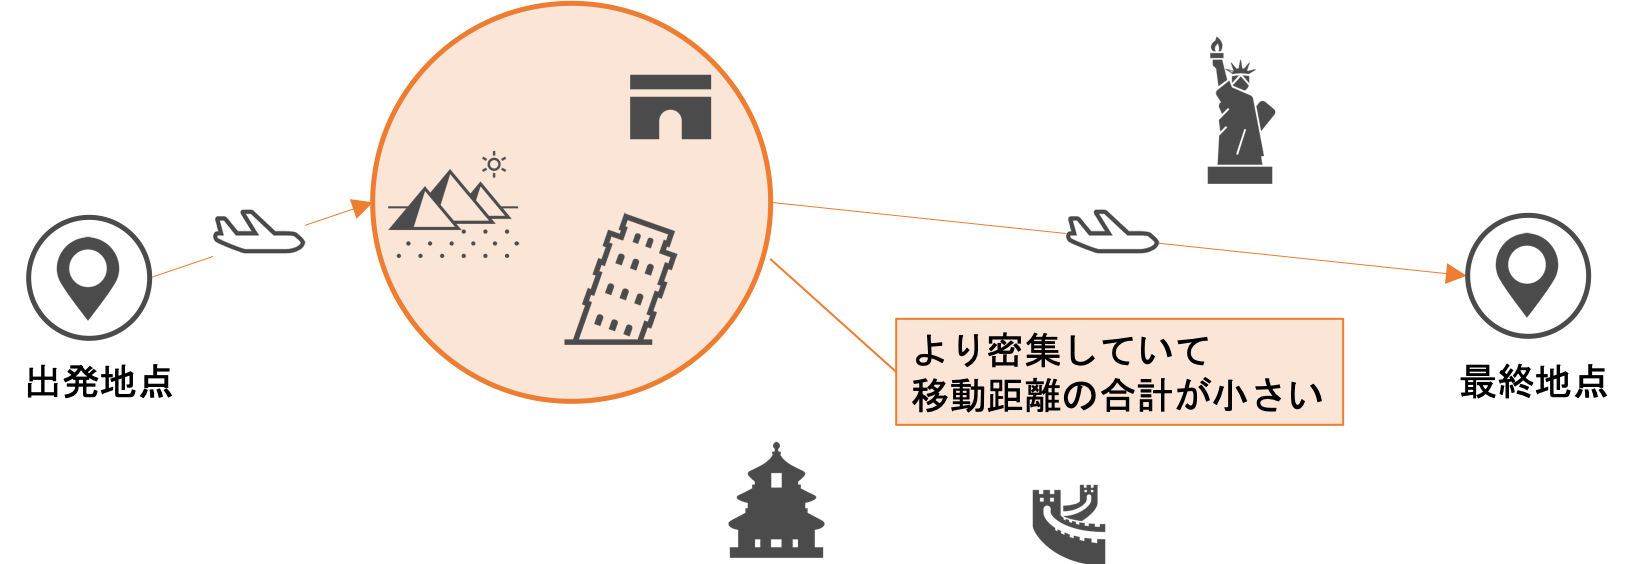
\includegraphics[width=8cm]{images/ex-sum.png}
    \caption{合計距離を最小とする例}
    \label{fig:ex-sum}
\end{figure}

図\ref{fig:ex-max1}は集合場所を決める際の例である。全員が集まりやすい場所であり、アクティビティが多くある地点を集合場所としたい。この場合各ユーザーの地点がクエリとなり、アクティビティスポットがデータセットとなる。提案手法ではクエリからクラスタまでに距離の最大値が最小となり、かつより密集しているクラスタを探索する。図\ref{fig:ex-max2}は解とならないクラスタの例である。クラスタの密集度は図\ref{fig:ex-max1}のクラスタと同程度だが、クエリとクラスタの距離の最大値が図\ref{fig:ex-max1}のクラスタの最大値よりも大きいため集合場所としては不適である。

\begin{figure}[H]
	\centering
    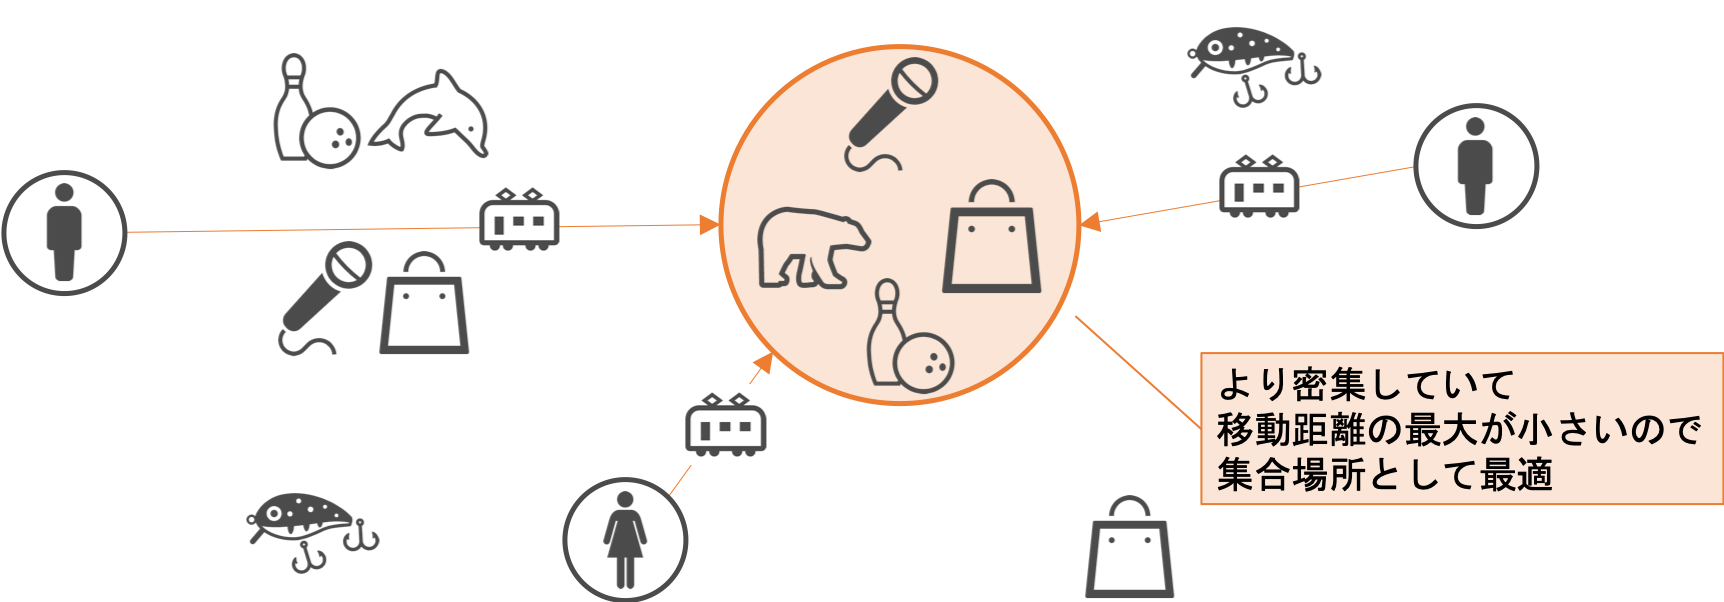
\includegraphics[width=8cm]{images/ex-max1.png}
    \caption{最大距離を最小とする例}
    \label{fig:ex-max1}
\end{figure}


\begin{figure}[H]
	\centering
    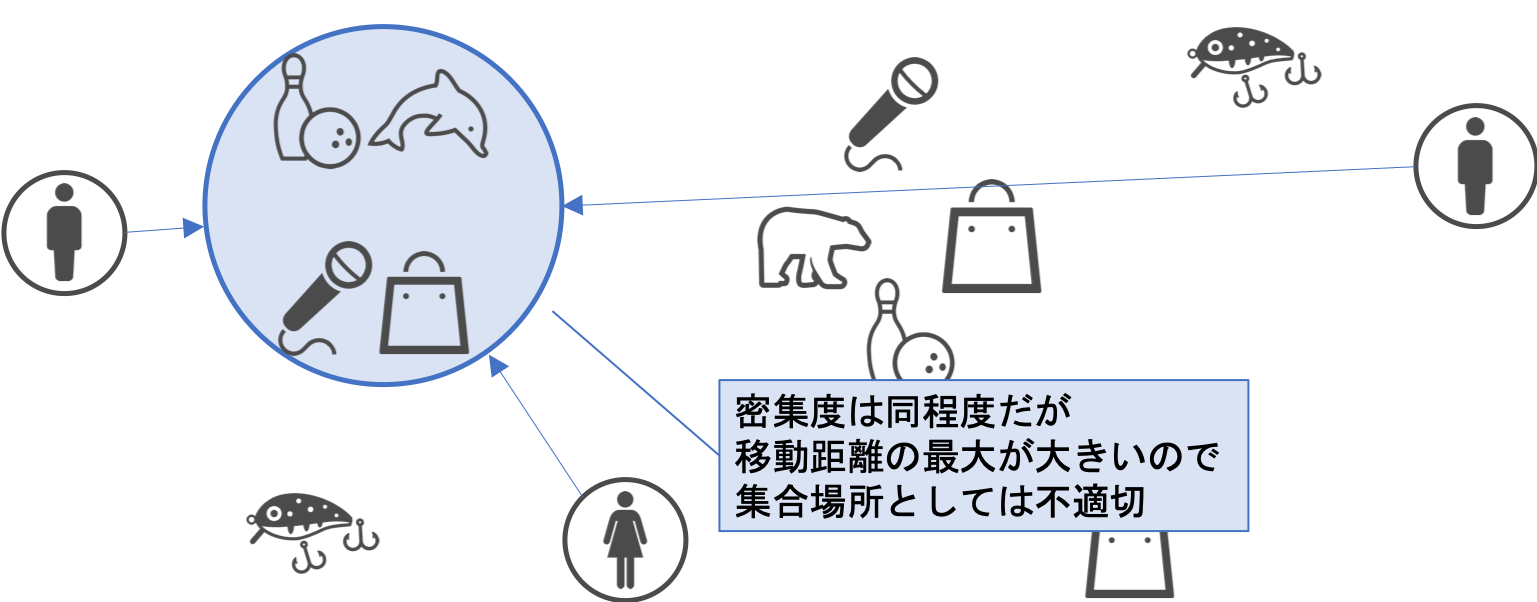
\includegraphics[width=8cm]{images/ex-max2.png}
    \caption{最大距離が最小になっていない例}
    \label{fig:ex-max2}
\end{figure}

\section{関連研究}

\subsection{R-Treeを用いた最近傍探索}
データベース管理システム、データマイニングおよび情報検索などの多くの分野において、基本的かつ重要な問題は、(k)最近傍クエリ問題(NN、またはkNN)である。クエリ点qとデータセットPが与えられると、NNはデータセットPからqに最も近い点を返す。 NNクエリを優れたパフォーマンスで解決するために多くの研究が行われてきた。最も一般的な解決策の1つは、Rツリーベースの処理である。\cite{cheung1998enhanced}\cite{hjaltason1999distance}。 R-tree\cite{R-tree}は、空間内の近接点を最小外接矩形(MBR)でグループ化し、MBRをツリー構造で管理する空間インデックスである。Hjaltason et al \cite{hjaltason1999distance}は、NNクエリを解決するためにRツリーを用いた最良優先探索を提案した。最良優先探索は次に探索する最も望ましいノードを選択するように探索をする。具体的には、クエリ点qまでの最小距離の順序でR木のMBRを含む優先待ち行列を作成する。

\subsection{複数問い合わせ点の集約最近傍}
従来のNNクエリのように単一点間の関係を評価するだけでは実際のアプリケーションでは活用できないため、さまざまな種類のNNクエリの変種が研究されてきた。 Taoらは複数のクエリ点までの最小集約距離を持つ点を取得するために、Aggregate Nearest Neighbor Queries(ANN)\cite{ANN}を提案した。 ANNは質問点群Qを入力し、Qまでの最小の集合距離を有する最も近い単一点を見出すことを目的としている。したがって、本研究はANNと比べてクエリを複数受け取る部分は合致しているが、クラスタを探索する点で異なっている。 Dengらは、Group nearest neighbor queries(GNG)\cite{GNG}を提案した。これは、クエリ群を入力に受け取り、グループを返す。GNGではレスポンスとなるグループの評価を各点のクエリからの距離で行なっているのに対して、本研究では点をクラスタと捉え、クラスタの密集度も評価に入れている部分で異なっている。
Nearest neighborhood search(NNH)\cite{NNH}はNNクエリを拡張し、クエリ点qに対して最近傍クラスタを返す。具体的には半径$\rho$の円の中心を返す。この円はkの点を含むクエリから最近傍の円である。Balanced Nearest Neighborhood Query(BNNH)\cite{BNNH}はNNHを拡張し、半径を固定長から変更可能にし、平滑パラメータを用いてクラスタの大きさとクエリ点からの距離のバランスを考慮した。


\section{提案手法}

ANN\cite{ANN}は複数クエリを入力にとり、単一点を出力としていた。またBNNH\cite{BNNH}は単一点を入力にとり、クラスタを出力としていた。本研究ではこれらの研究では探索できない、複数クエリを入力として、出力をクエリの最近傍のクラスタとする。
BNNH\cite{BNNH}ではクラスタを円と定義し、密集度を円の半径としていたが、円を形成するのに計算が必要な上に、クラスタ内部のデータの偏りを検知できない問題があった。本研究ではクラスタの形を円に限定せず、クラスタ内の分散で密集度を評価することで、計算量の削減とより密集したクラスタを探索することを実現している。

以下の説明で使用する変数について表\ref{tab:var}に示す。ユーザーからクエリ群$Q$、クラスタサイズ$k$、クラスタの距離と密集度の好みのバランスを設定する$\alpha, \beta$が与えられ、最近傍のクラスタを返す。

\begin{table}[htb]
  \begin{center}
    \begin{tabular}{|l|l|} \hline
      要素名 & 説明 \\ \hline \hline
      $p, P$ & 点, 点のクラスタ \\ \hline
      $q, Q$ & クエリ点, クエリ群 \\ \hline
      $C, V_C$ & クラスタ, クラスタ内の分散 \\ \hline
      $O_C$ & クラスタの重心 \\ \hline
      $dist(p,q)$ & 点$p$と点$q$のユークリッド距離 \\ \hline
      $\alpha, \beta$ & ユーザー定義の平滑パラメータ \\ \hline
      $k$ & ユーザー定義のクラスタサイズ \\ \hline
      $\Delta(C,Q)$ & $C$と$Q$の複合類似度 \\ \hline
      $MBR$ & R-treeの最小外接矩形 \\ \hline
      $n$ & グリッドを用いた手法におけるセル数 \\ \hline
    \end{tabular}
    \caption{記号の説明}
    \label{tab:var}
  \end{center}
\end{table}

\subsection{集約最近傍}
クエリが複数になることにより、クエリ群$Q$と点$p$の最近傍について定義が必要になる。本研究では"合計"、"最大"を最近傍の指標として挙げる。
\subsubsection{合計値の集約最近傍}
各クエリからクラスタまでの距離の合計が最小となるクラスタを最近傍とする。図\ref{fig:ex-sum}で示した例のように、ユーザーは1人でクエリとして経路の地点を設定することで移動距離が最小となるような問題を解決できる。点$p$とクエリ$Q$の集約距離を求める式を(\ref{equ:f-sum})に示す。
\begin{equation}
\label{equ:f-sum}
f_{sum}(p,Q) = \sum_{i=1}^{n} dist(p,q_i)
\end{equation}

\subsubsection{最大値の集約最近傍}
各クエリからクラスタまでの距離の最大値が最小となるクラスタを最近傍とする。図\ref{fig:ex-max1}で示した例のように、クエリがユーザーの位置で、集合場所を決める際に中間地点を選択する問題を解決できる。
\begin{equation}
\label{equ:f-max}
f_{max}(p,Q) = max_{i=1}^{n} dist(p,q_i)
\end{equation}

\subsection{クラスタ内分散}
クラスタの密集度をクラスタ内分散$V$で表す。点$p_1, \cdots p_n$が構成するクラスタ$P$の重心が$G_P$の時、$P$の分散を求める式を以下に示す。
\begin{equation}
\label{equ:w}
V_P = \frac{1}{|P|} \sum_{i=1}^{n} \{dist(p_i, G_P)\}^2 
\end{equation}

\subsection{クラスタの評価関数}
クラスタの密集度はクラスタ内分散$V_C$で表すとする。また、クエリとクラスタの距離の評価は式(\ref{equ:f-sum})-(\ref{equ:f-max})で行う。BNNH\cite{BNNH}で提案されている合成関数を変形し、本研究で用いる評価関数$\Delta(.)$を以下に示す。
\begin{equation}
\label{equ:f-delta}
\Delta(C,Q) = \alpha \cdot f(O_C, Q) + \beta \cdot V_C\ \
\end{equation}

式(\ref{equ:f-delta})を用いて平滑パラメータ$\alpha, \beta$の値を変えることによってユーザーの好みを反映できる。例えば$\alpha>\beta$の場合はクラスタの位置が近い方が好ましいことを表し、$\alpha<\beta$の場合はクラスタの密度が高い方が好ましいことを表し、$\alpha=\beta$の場合はクラスタの位置と密度が同程度重要であることを表す。図\ref{fig:ex-delta}には3つのクラスタ$R_1$、$R_2$、$R_3$がある。この例では$R_2$がクラスタの密度が一番大きく、クエリに近いので解となる。$R_1$と$R_3$を比較すると密度は$R_3$の方が高いが、クエリとの距離は$R_1$の方が小さい値になっている。このような場合にクラスタを単純比較できないため、評価関数を用いて比較を行う。

\begin{figure}[H]
	\centering
    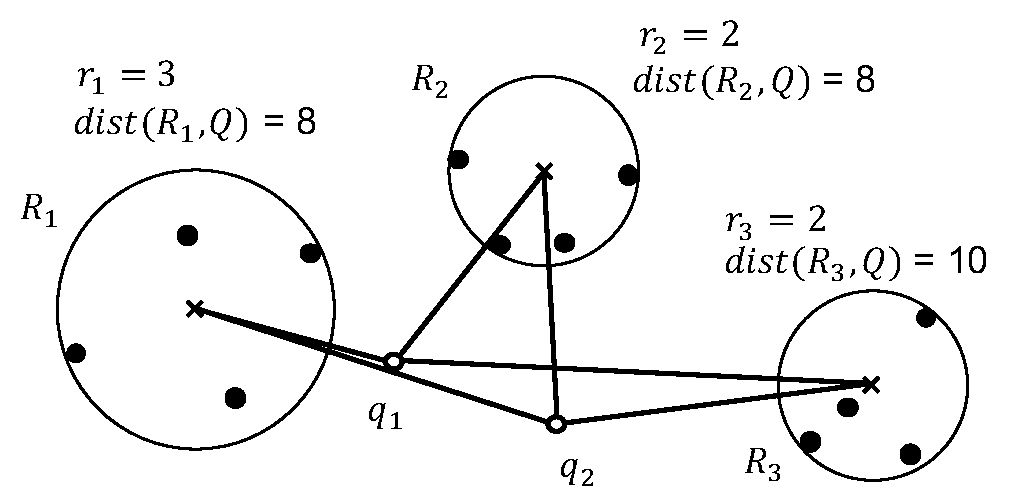
\includegraphics[width=8cm]{images/ex-delta.pdf}
    \caption{クラスタの距離と密集度の関係}
    \label{fig:ex-delta}
\end{figure}

\subsection{フィルタリング}
全てのデータ点$p$に対してクラスタを作成し、$\Delta(.)$の値を計算することはとても非効率である。これを省略するために、計算を行う前にフィルタリングを行う。
評価式の両辺を$\alpha+\beta$で割ると次の式となる。
\begin{equation}
\label{equ:filter-1}
\frac{\Delta(C,Q)}{\alpha+\beta} = \frac{\alpha}{\alpha+\beta} \cdot f(O_C, Q) + \frac{\beta}{\alpha+\beta} \cdot V_C\ \
\end{equation}

$\alpha < \beta$の時、
$$\frac{\alpha}{\alpha+\beta}  < 0.5, \frac{\beta}{\alpha+\beta} > 0.5$$
である。

$\alpha + \beta < 1$の時、式(\ref{equ:f-delta})を変形し、以下の式を導出できる。
\begin{equation}
\label{equ:filter1}
\frac{\alpha + \beta}{\alpha}\cdot \Delta(C,Q) < f(O_C, Q) + V_C\ \  (\alpha < \beta)
\end{equation}

現時点で最善の解$C_1$、$C_1$に属さない点$p$、$p$と他の任意の点を持つクラスタ$C_2$を考えると、
\begin{equation}
\label{equ:filter2}
f(p,Q) \leq f(O_{C_2},Q)+V_{C_2} < \frac{\alpha + \beta}{\alpha}\cdot \Delta(C_2,Q)
\end{equation}

$\frac{\alpha + \beta}{\alpha} \cdot \Delta(C_1,Q) < f(p,Q)$が成り立つとき、式(\ref{equ:filter2})より$\Delta(C_1,Q) < \Delta(C_2,Q)$が成り立つ。

これより、$\alpha < \beta$のとき、クエリ群$Q$とその時点での最善解であるクラスタ$C$を考えたときに、ある点$p$の$f(p,Q)$が$\frac{\alpha + \beta}{\alpha} \cdot \Delta(C,Q)$を超えた時に、点$p$は最善解には含まれないといえる。
これを一般化すると以下の条件を満たす時に点$p$はフィルタリングされる。
\begin{equation}
\label{equ:filter-final}
f(p,Q) > \frac{\alpha + \beta}{min(\alpha, \beta)} \cdot  \Delta(C,Q)
\end{equation}

\subsection{ポイントベースの手法}
以上の式を用いてクラスタを探索する手法を示す。まずはシンプルに探索するポイントペースの手法である。これは各データセットの点に対して$k-1$点の最近傍点を探し出し、クラスタを計算する。このクラスタの評価関数の値がその段階での最善解よりも良ければ解として更新する。クラスタを作成する前に式(\ref{equ:filter-final})を用いてフィルタリングを行う。ポイントベースの手法の擬似アルゴリズムをAlgorithm\ref{alg:point}に示す。

\begin{algorithm}                      
\caption{ポイントベースの手法}         
\label{alg:point}
\begin{algorithmic}[1]                  
\renewcommand{\algorithmicrequire}{\textbf{Input:}}
\renewcommand{\algorithmicensure}{\textbf{Output:}}
\REQUIRE $P,Q,k,\alpha, \beta$
\ENSURE $C$
\STATE $bound \xleftarrow[]{} \infty$
\STATE $C \xleftarrow[]{} \emptyset$
\FOR{$each\ p_i \in P$}
\IF{$f(p_i,Q)<bound$}
\STATE $pSet \xleftarrow{} p_i$ and its $k-1$ nearest points
\STATE $C_t \xleftarrow{}$ create Cluster with $pSet$
\IF{$\Delta(C_t,Q)<\Delta(C,Q)$}
\STATE $C \xleftarrow{} C_t$
\STATE update $bound$ with $\Delta(C_t,Q)$
\ENDIF
\ENDIF
\ENDFOR
\RETURN $C$
\end{algorithmic}
\end{algorithm}

\begin{algorithm}                      
\caption{R-treeを用いる手法}         
\label{alg:r-tree}
\begin{algorithmic}[1]                  
\renewcommand{\algorithmicrequire}{\textbf{Input:}}
\renewcommand{\algorithmicensure}{\textbf{Output:}}
\REQUIRE $P,Q,k,\alpha, \beta$
\ENSURE $C$
\STATE $p_a \xleftarrow[]{}$ the nearest point to q from P.
\STATE $pSet \xleftarrow{} p_a$ and its $k-1$ nearest points
\STATE $C \xleftarrow[]{}$ create Cluster with pSet
\STATE $bound \xleftarrow[]{} $calculate the filter condition with $\Delta(C,Q)$
\STATE $heep \xleftarrow[]{} Rtree.root$
\WHILE{$heap$ is not empty}
\STATE $E \xleftarrow[]{}heap.front()$
\IF{$mindit(E,Q)<bound$}
\IF{$E$ is none-leaf node}
\STATE $heap \cap E.children$
\ENDIF
\IF{$E$ is leaf node}
\FOR{each $p \in E$}
\IF{$dist(p_i, Q) < bound$}
\STATE $pSet \xleftarrow{} p_i$ and its $k-1$ nearest points
\STATE $C_t \xleftarrow{}$ create Cluster with $pSet$
\IF{$\Delta(C_t,Q)<\Delta(C,Q)$}
\STATE $C \xleftarrow{} C_t$
\STATE update $bound$ with $\Delta(C_t,Q)$
\ENDIF
\ENDIF
\ENDFOR
\ENDIF
\ENDIF
\ENDWHILE
\RETURN $C$
\end{algorithmic}
\end{algorithm}

\subsection{R-treeを用いる手法}
ポイントベースの手法ではフィルタリングが点単位であり、R-treeの$MBR$単位でフィルタリングを行えば効率的にフィルタリングができ、計算量の減少が見込める。データセットをR-tree上に配置し、$Q$も$MBR$として配置する。各ノードと$Q$の距離でフィルタリングを行うことで、一度にフィルタリングを行うことができる。R-treeを用いる手法の擬似アルゴリズムをAlgorithm\ref{alg:r-tree}に示す。

\begin{figure}[H]
	\centering
    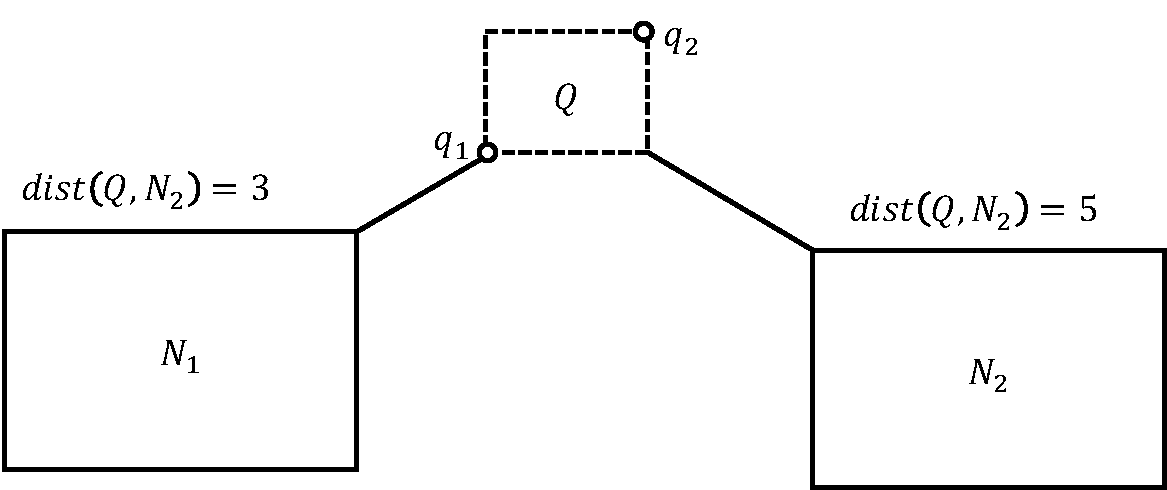
\includegraphics[width=8cm]{images/sol-r-tree.pdf}
    \caption{R-treeを用いる手法}
    \label{fig:sol-r-tree}
\end{figure}

\subsection{グリッドを用いる手法}
R-treeのを用いた手法の欠点は、走査が行われる際に毎回ルートノードから開始される点が挙げられる。また、NN探索のフィルタリングにおいて、クエリ点近くから探索を行うと、フィルタリングの閾値が小さくなり、フィルタリング量が多くなることが報告されている\cite{BNNH}。これらより、既存研究\cite{BNNH}と同様にデータセットを2次元空間のグリッドに配置する。クエリ点が1つの時の例を図\ref{fig:sol-grid-filter}に示す。クエリ$q'$が存在するセルを特定し、その周辺のセルを探索することができる。これによって効率的に探索が行うことができる。閾値は図\ref{fig:sol-grid-filter}では点線の円で表され、点線の円の中のセルのみ探索を行えば良いということになる。本研究では複数クエリの際に探索するセルの起点をクエリ群の重心とする。グリッドを用いる手法の擬似アルゴリズムをAlgorithm\ref{alg:grid}に示す。

\begin{algorithm}                      
\caption{グリッドを用いる手法}         
\label{alg:grid}
\begin{algorithmic}[1]                  
\renewcommand{\algorithmicrequire}{\textbf{Input:}}
\renewcommand{\algorithmicensure}{\textbf{Output:}}
\REQUIRE $P,Q,k,\alpha, \beta$
\ENSURE $C$
\STATE $p_a \xleftarrow[]{}$ the nearest point to q from P.
\STATE $pSet \xleftarrow{} p_a$ and its $k-1$ nearest points
\STATE $C \xleftarrow[]{}$ create Cluster with pSet
\STATE $bound \xleftarrow[]{} $calculate the filter condition with $\Delta(C,Q)$
\STATE $nextCells \xleftarrow[]{} $ get surround cells of $q$
\WHILE{nextCells locate in $bound$}
\STATE $pNext \xleftarrow[]{}$ retrieve newarest point to $q$ from $nexCells$
\STATE $pSet \xleftarrow[]{} pNext$ and its $k-1$ nearest points
\STATE $C_t \xleftarrow{}$ create Cluster with $pSet$
\IF{$\Delta(C_t,Q)<\Delta(C,Q)$}
\STATE $C \xleftarrow{} C_t$
\STATE update $bound$ with $\Delta(C_t,Q)$
\ENDIF
\STATE $nextCells \xleftarrow[]{} $ the next round of cells
\ENDWHILE
\RETURN $C$
\end{algorithmic}
\end{algorithm}


\begin{figure}[H]
	\centering
    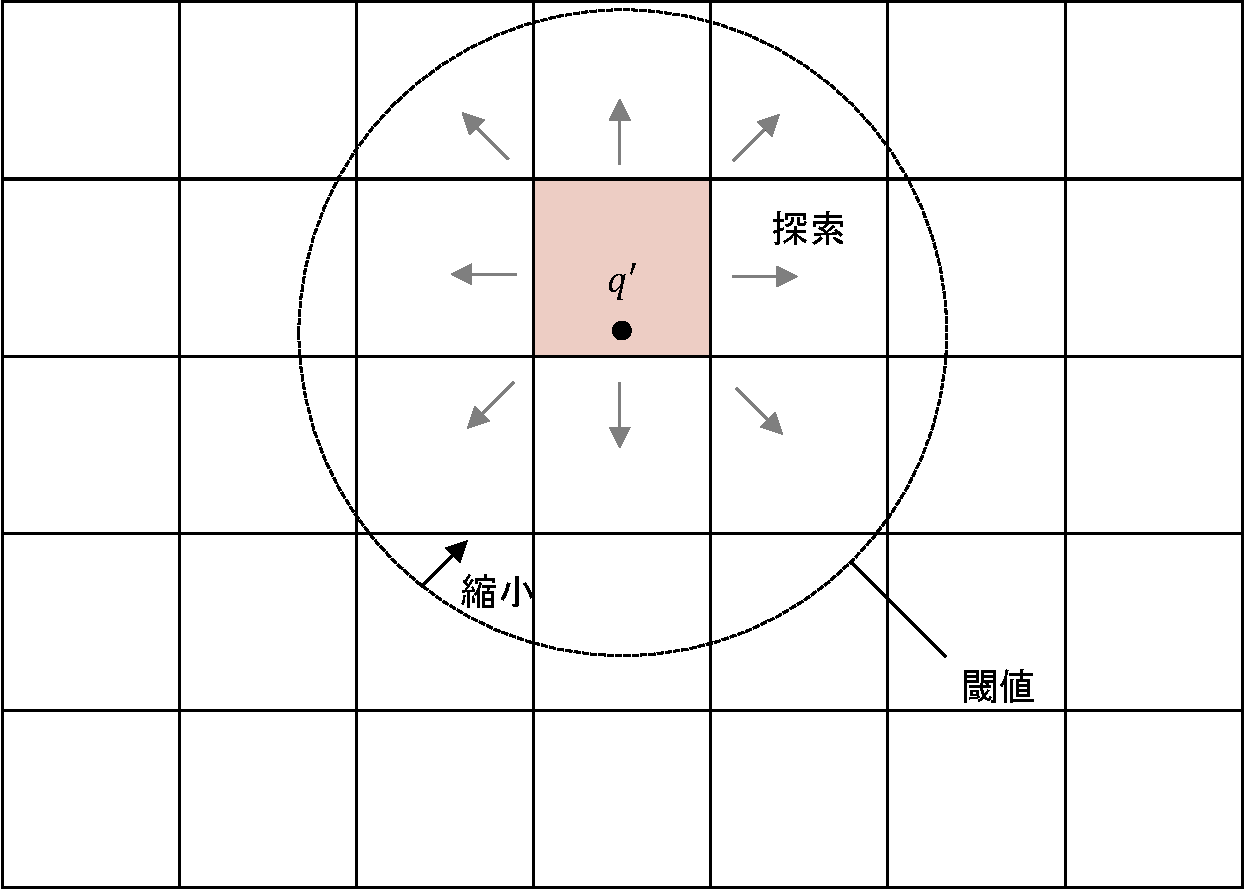
\includegraphics[width=8cm]{images/sol-grid-filter.pdf}
    \caption{グリッドを用いる際のフィルタリング}
    \label{fig:sol-grid-filter}
\end{figure}

\section{実験}
\subsection{実験環境}
提案手法の有用性を示すために、実験を行った。実験環境をいかに示す。
\begin{itemize}
  \item OS: macOS 10.15.2 (19C57)
  \item CPU: 2.7 GHz Intel Core i5
  \item Memory: 16 GB 1867 MHz DDR3
  \item 開発言語: C++
\end{itemize}

\subsection{データセット}
実データと合成データを用いて実験を行った。実データはアメリカ国勢調査TIGERプロジェクト\cite{chorochronos}から取得したデータNE(123,593点)から一様乱数を用いて1万点を抜き出し、データセットを作成した。合成データは一様分布に基づくデータセットを作成し、使用した。

\subsection{パラメータ}
クエリはデータセットからランダムに選択した。出力結果となるクエリサイズ$k$のデフォルト値は50、平滑パラメータ$\alpha, \beta$は共に0.5、グリットを用いる手法で分割するグリット数は$128^2$である。全ての実験結果は10回の試行の平均を用いている。

\subsection{実験結果}
平滑パラメータ$\alpha$を変化させた結果を図\ref{fig:sum-alpha}と図\ref{fig:max-alpha}に示す。集約距離をどちらに設定してもグリッドを用いた手法が他の2手法に比べて高速であることがいえる。これはグリッドを用いた手法ではクエリの近くから探索するので、フィルタリングに用いる閾値が早期に適切に設定され、フィルタリング量が大きかったためである。

2つの集約距離に一貫して、$\alpha$が0.5を超えると処理時間がスパークする傾向にあった。これは評価式において、前半の項の大きさが後半の項と比較して大きく、閾値が$\beta$に比べて$\alpha$に依存している傾向にあるからだと考えられる。

\begin{figure}[H]
	\centering
     \fbox{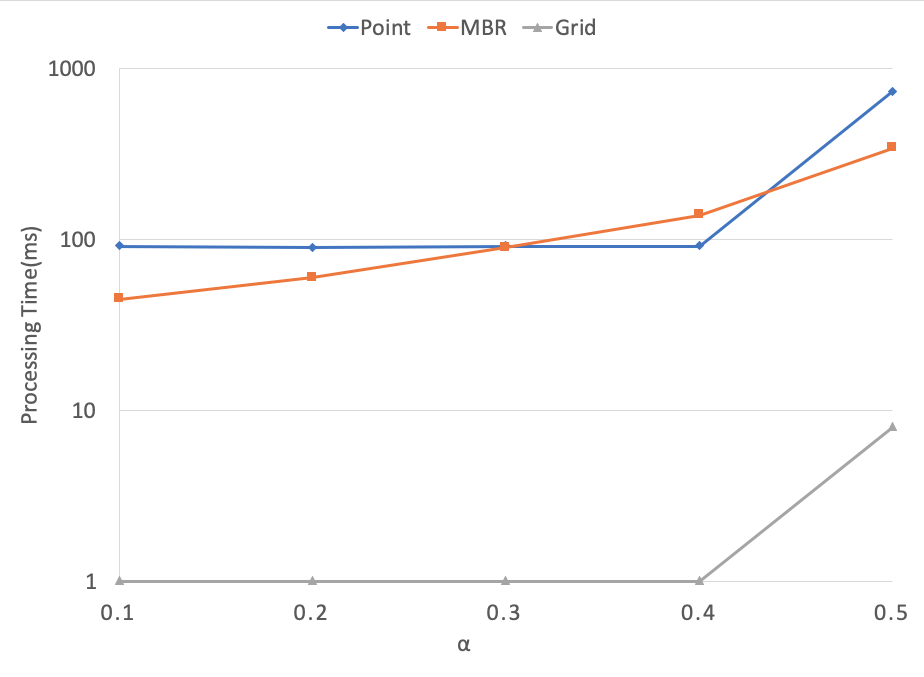
\includegraphics[width=7cm]{images/experiment/variance/sum-alpha-beta.png}}
    \caption{$f=sum$, NE, $\mid$P$\mid$ = 123,593, $\beta$ = 0.5, k = 50, $\mid$Q$\mid$ = 5, n = $128^2$}
    \label{fig:sum-alpha}
\end{figure}

\begin{figure}[H]
	\centering
    \fbox{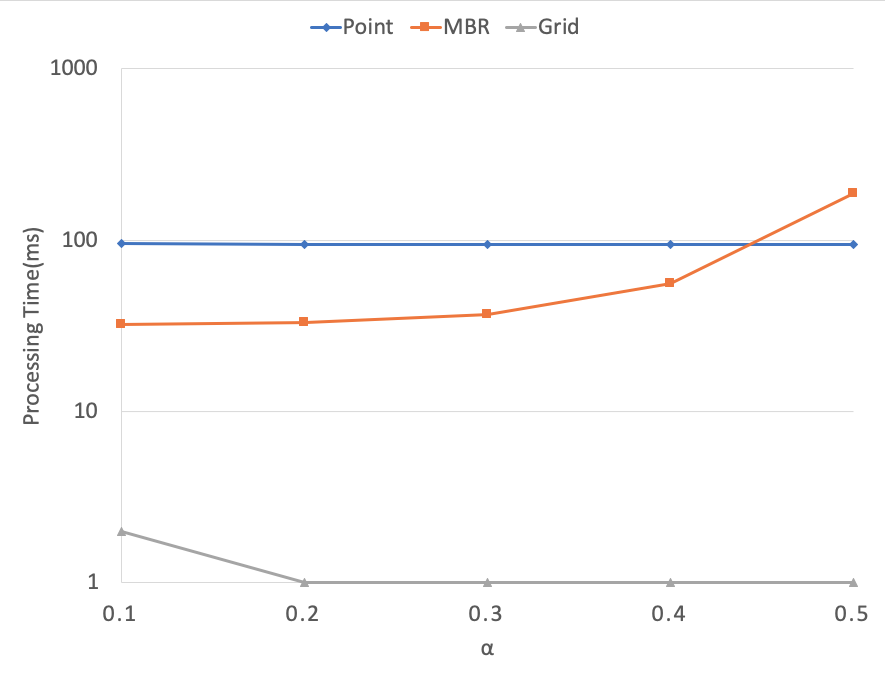
\includegraphics[width=7cm]{images/experiment/variance/max-alpha-beta.png}}
    \caption{$f=max$, NE, $\mid$P$\mid$ = 123,593, $\beta$ = 0.5,  k = 50, $\mid$Q$\mid$ = 5, n = $128^2$}
    \label{fig:max-alpha}
\end{figure}

クエリサイズを変化させた結果を図\ref{fig:sum-querySize}と図\ref{fig:max-querySize}に示す。集約距離合計と最大においてグリッドを用いた手法が最速になった。グリッドを用いた手法ではクエリサイズが大きくなるほど速くなる結果となった。集約距離を最大に設定すると、ポイントベースとR-treeを用いた手法では集約距離合計の場合よりも速い結果となった。これはフィルタリングに用いる閾値と比較する値が、集約距離合計の際にはクエリからの距離の平均であるのに対して、集約距離合計の際にはクエリからの距離からの最大値であるので、フィルタリング量が大きかったと考えられる。

\begin{figure}[H]
	\centering
    \fbox{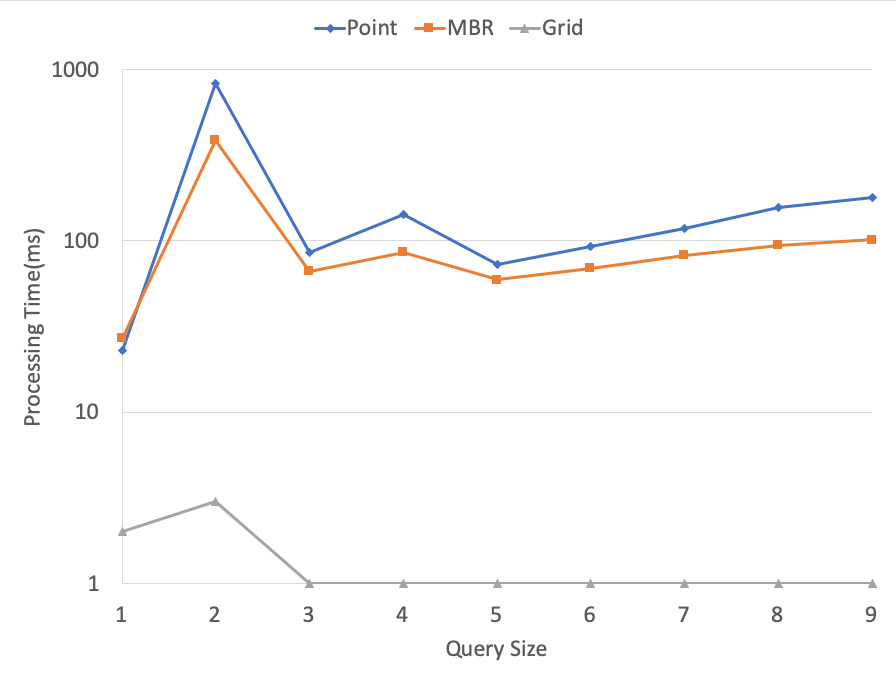
\includegraphics[width=7cm]{images/experiment/variance/sum-querySize.png}}
    \caption{$f=sum$, NE, $\alpha$ = 0.5 , $\beta$ = 0.5 , $\mid$P$\mid$ = 10,000, k = 50, n = $128^2$}
    \label{fig:sum-querySize}
\end{figure}

\begin{figure}[H]
	\centering
    \fbox{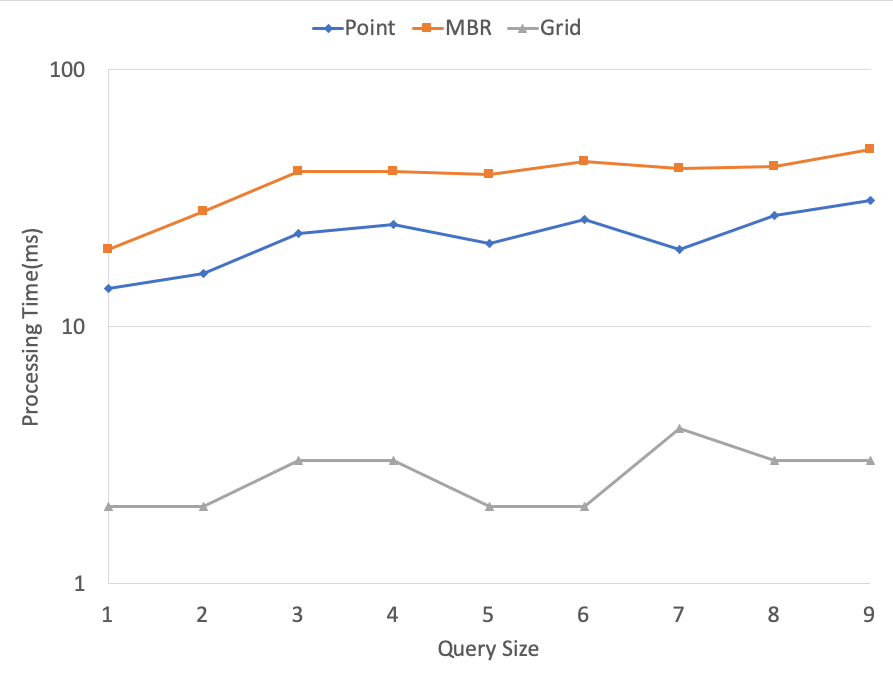
\includegraphics[width=7cm]{images/experiment/variance/max-querySize.png}}
    \caption{$f=max$, NE, $\alpha$ = 0.5 , $\beta$ = 0.5 , $\mid$P$\mid$ = 10,000, k = 50, n = $128^2$}
    \label{fig:max-querySize}
\end{figure}

クラスタサイズを変化させた結果を図\ref{fig:sum-clusterSize}と図\ref{fig:max-clusterSize}に示す。両方の集約距離でグリッドが最速となった。

\begin{figure}[H]
	\centering
    \fbox{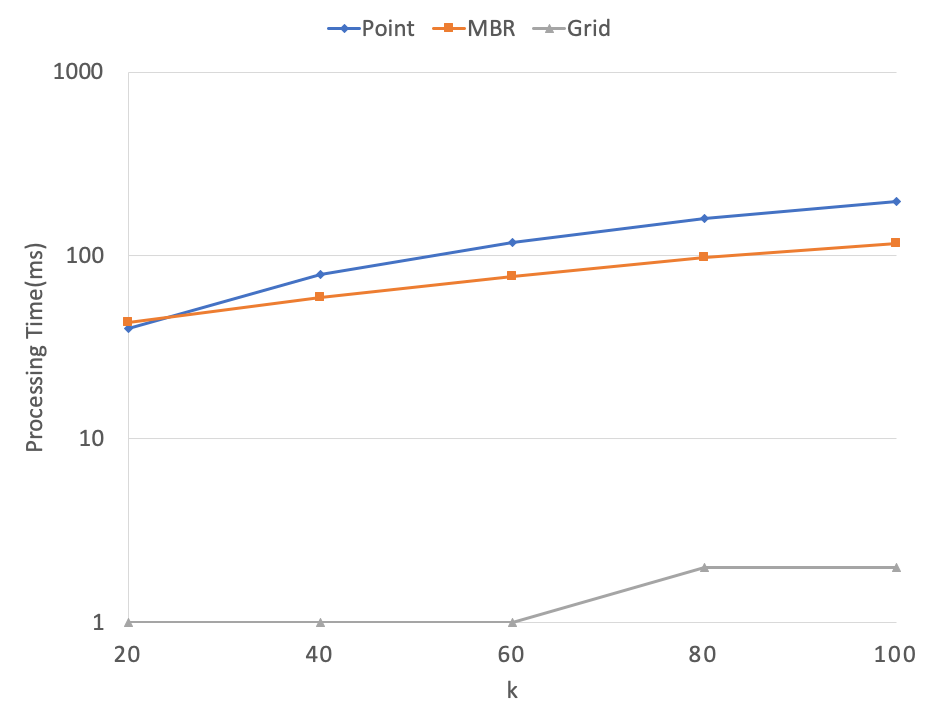
\includegraphics[width=7cm]{images/experiment/variance/sum-clusterSize.png}}
    \caption{$f=sum$, NE, $\alpha$ = 0.5 , $\beta$ = 0.5 , $\mid$P$\mid$ = 10,000, $\mid$Q$\mid$ = 5, n = $128^2$}
    \label{fig:sum-clusterSize}
\end{figure}

\begin{figure}[H]
	\centering
    \fbox{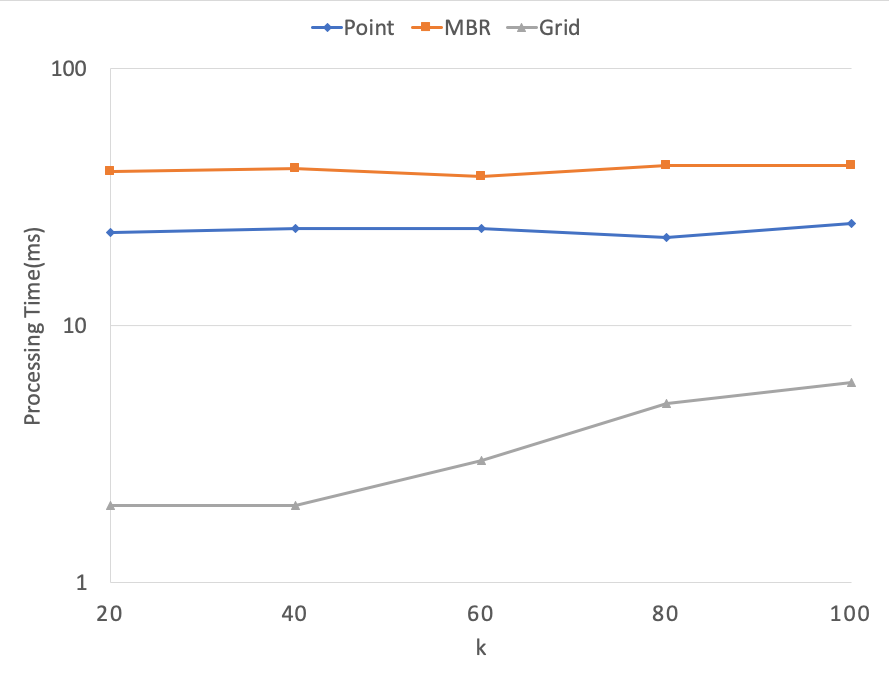
\includegraphics[width=7cm]{images/experiment/variance/max-clusterSize.png}}
    \caption{$f=max$, NE, $\alpha$ = 0.5 , $\beta$ = 0.5 , $\mid$P$\mid$ = 10,000, $\mid$Q$\mid$ = 5, n = $128^2$}
    \label{fig:max-clusterSize}
\end{figure}

データサイズを変化させた結果を図\ref{fig:sum-dataSize}と図\ref{fig:max-dataSize}に示す。グリッドを用いた手法が最速となった。3手法とも線形に処理時間が増えていることがわかる。

\begin{figure}[H]
	\centering
    \fbox{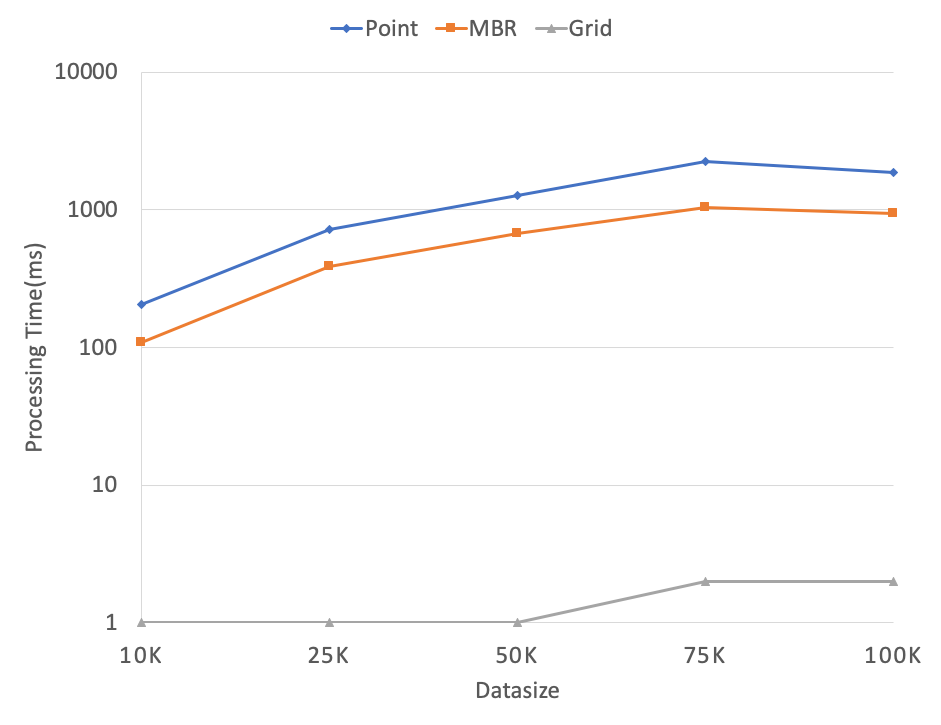
\includegraphics[width=7cm]{images/experiment/variance/sum-dataSize.png}}
    \caption{$f=sum$, UN, $\alpha$ = 0.5 , $\beta$ = 0.5 ,k = 50, $\mid$Q$\mid$ = 5, n = $128^2$}
    \label{fig:sum-dataSize}
\end{figure}

\begin{figure}[H]
	\centering
    \fbox{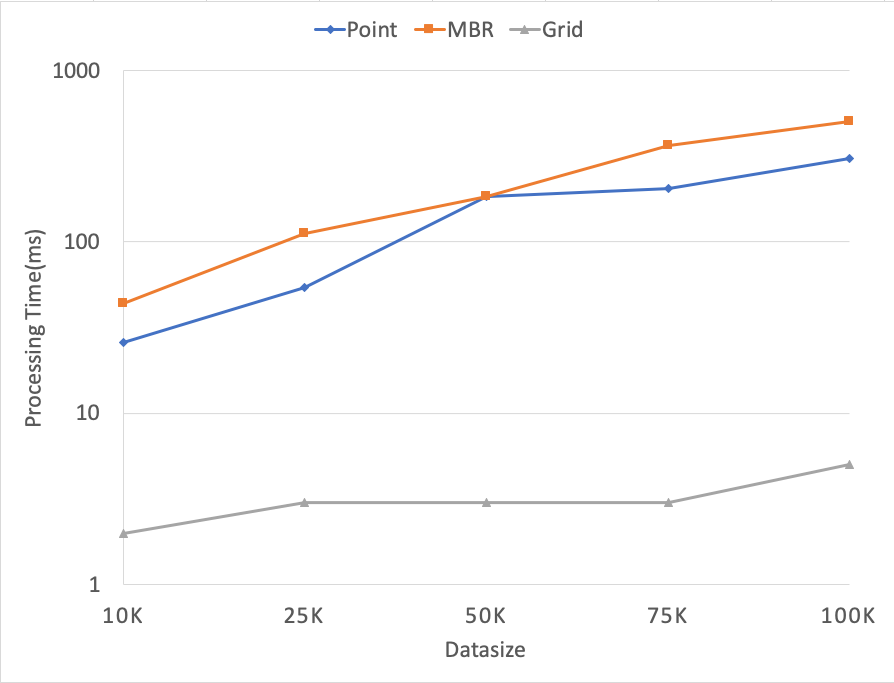
\includegraphics[width=7cm]{images/experiment/variance/max-dataSize.png}}
    \caption{$f=max$, UN, $\alpha$ = 0.5 , $\beta$ = 0.5 ,k = 50, $\mid$Q$\mid$ = 5, n = $128^2$}
    \label{fig:max-dataSize}
\end{figure}

\section{結論と今後の課題}
最近傍クラスタを見つけることは、クエリ処理とデータマイニングにおいて重要な問題である。既存研究では複数のクエリの最近傍のクラスタを探索することはできなかった。本研究では集約距離を定義することで、複数クエリの最近傍のクラスタ探索を実現した。クラスタを探索する手法として、ポイントベース、R-tree、グリッドを用いる3つの手法を提案した。合成データと実データを用いた実験では集約距離合計ではグリッドを用いた手法が最も効率が良いことを示した。

今後の課題として、平滑パラメータの値によってパフォーマンスが落ちる傾向にあり、これを解消したいと考えている。

\section*{謝辞}
本研究はJSPS科研費JP19K12114の助成を受けたものである.

%\vspace{30mm} <- 文献が本文と近すぎるときは適宜利用してください.
\vspace{2em}

\bibliography{main} % bibFileName
\bibliographystyle{unsrt}  % bibStyleName


\end{document}
